The Standard Model (SM) of particle physics, a gauge quantum field theory was developed to describe three fundamental forces in the universe: strong force, weak force and the electromagnetic force and simultaneously, classifies elementary particles.\\
To explain how the gauge bosons acquired mass in SM, a complex scalar doublet field which self-interacted and allowed spontaneous electroweak symmetry breaking (EWSB), was introduced, with the inclusion of a new particle known as \q{Higgs Boson}. The following chapter will give an overview of the theory of Standard Model of particle physics, the production and decay modes of Higgs along with a brief description of the golden channel. Finally, the chronicle searches by LHC experiments to find Higgs boson.

\section{Particle Physics}
\subsection{Building Blocks of Particle Physics}
Elementary particles are the basic units of Standard Model. The elementary particles are split into two spin families: fermions (spin = $\frac{1}{2}$) and bosons (spin = 1). The Standard Model elementary particles are matter particles (leptons and  quarks), the force carriers ($W, Z,$ \Pphoton, \Pgluon) and the Higgs boson. Leptons and quarks are divided into three generations as they are spin $\frac{1}{2}$ fermions. The particles in each generation have different flavour and mass. Generation 1 contains the lightest and the most stable particles while the heaviest and most unstable one are classified in the second and the third generations. The fermion's classification is shown in Table.\ref{tab:ep} \cite{<PDG>}. The bar above the symbol of the particle represents anti-particle with an opposite quantum number.\\ 
Leptons exist as free particles in nature and interact by electroweak (EWK) interaction, while quarks in hadrons interact by means of both strong and EWK interactions. A pair of quark with an anti-quark forms a meson which is a bosonic hadron while 3 (anti)quarks form (anti)baryon which is a fermionic hadron.\\
Standard model force carriers consist of; massless photons (\Pphoton) which mediates the electromagnetic (EM) force, three gauge bosons (\PZ, \PWpm) which mediate the weak force and 8 massless gluons (\Pgluon) are conducive for the strong force. Higgs boson (\PHiggs) was the last discovered, a heavy scalar particle which mediates the Higgs field. Table.\ref{tab:boson}  \cite{<PDG>} shows some properties of force mediators.
\begin{table}[]
    \centering
    \begin{tabular}{|c|l|l|l|l|l|l|}
    \hline
         Generation & Flavour& Symbol & Family & Mass(GeV) & Charge(e) & Interaction\\
     \hline 
     \hline
         \multirow{2}{*}{I} & electron &\Pe & lepton & 0.000511 & -1 & EM,Weak \\ 
         & \Pe neutrino &  \Pnue &lepton& $<1.18^{-8}$ & 0 & Weak\\ 
         \hline
         \multirow{2}{*}{II} & muon & \Pmu  & lepton & 0.106 & -1 & EM, Weak\\
         & \Pmu neutrino& \Pnum & lepton & $<0.002$ & 0 & Weak\\
         \hline 
         \multirow{2}{*}{III} & tau & \Ptau & lepton& 1.777 & -1 & EM, Weak\\
         & \Ptau neutrino & \Pnut & lepton & $<0.02$ & 0 & Weak\\
         \hline 
         \multirow{2}{*}{I} & up &\Pup & quark & 0.002 & $ \frac {2}{3}$ & All \\
         & down & \Pdown & quark &0.005 & $-\frac{1}{3}$ & All \\
         \hline
         \multirow{2}{*}{II} & charm & \Pcharm & quark & 1.275 & $ \frac {2}{3}$ & All  \\
         & strange &\Pstrange & quark & 0.095 & $-\frac{1}{3}$ & All\\
         \hline 
         \multirow{2}{*}{III} &top & \Ptop & quark & 173 & $ \frac {2}{3}$ & All\\
         & bottom & \Pbottom & quark &4.18 & $-\frac{1}{3}$ & All\\
         \hline
    \end{tabular}
    \caption{Distribution of Fermions}
    \label{tab:ep}
\end{table}

\begin{table}[h]
\centering
\begin{tabular}{| l | l | l | l | l| l|}
\hline
\multicolumn{6}{|c|}{FORCE MEDIATORS} \\
\hline
\hline
Name & Symbol & Spin & Charge(e) & Mass[GeV] & Mediates \\
\hline
Photon & \Pphoton & 1 & 0 & 0 & EM \\
$\PWpm$ Boson & \PWpm & 1 & $\pm1$ & 80.4 & Weak \\
$Z^0$ Boson& \PZzero & 1 & 0 & 91.2 & Weak \\
gluons & \Pgluon & 1 & 0 & 0 & Strong \\
Higgs boson & \PHiggs & 0 & 0 & 125 & Higgs Field\\
graviton & $G$ & 2 & 0 & 0 & Gravitation \\
\hline
\end{tabular}
\caption{Distribution of Force Carriers}
\label{tab:boson}
\end{table}

\subsection{Quantum Field Theory of Particle Physics}
All building blocks are quantum fields in Standard Model which define the whole space time. The fields are given below;
\begin{itemize}
    \item Field of fermions for matter, $\Ppsi$.
    \item Fields of EWK boson, $W_1, W_2, W_3$ and B;
    \item Fields of gluons $G_a$,
    \item Field of Higgs, $\Pphi$.
\end{itemize}

The fundamental fields and fluctuations in quantum states are determined with Lagrangian density $\mathcal{L}$. The Standard Model does not vary under local gauge symmetry, where parameter conversion is a function of points in space that the particular field spans. The gauge group describing the Standard Model is $SU(3)_C \times SU(2)_L \times U(1)_Y$ where the index $C$ represents colour, $L$ represents left-handed and $Y$ is for hypercharge, respectively. The $SU(3)_C$ acts on $G_a$, $SU(2)_L$ acts on $W$ and $\Pphi$, and $U(1)_Y$ acts on $B$ and $\Pphi$.\\
The next section will give an overview of the conventions used to construct strong interaction through local gauge symmetry, based on Quantum Chromodynamics (QCD). Glashow-Weinberg-Salam \cite{<gws>} used an identical formalism for EWK theory which unifies electromagnetic and weak interactions, built upon weak hypercharge and weak iso-spin group represented by $U(1)_Y \times SU(2)_L$.\\

\textbf{QUANTUM COLOR THEORY}\\

Quantum Chromodynamics (QCD) expresses the interaction amidst gluons and quarks, built upon $SU(3)_C$ symmetry group. Quantum number is the colour that can take three possibilities: green, red and blue. $SU(3)_C$ symmetry group is a non-commutative group which consists of 8 Gell-Mann matrices $\frac{\lambda_a}{2}$, $a$=generator number, to the corresponding 8 generators. The Dirac Lagrangian is defined as:
\begin{equation}
    \mathcal{L}_{QCD}=\Paq_{f}(i\Pgg^{\mu}\partial_\mu-m)\Pquark_f.
\end{equation}
As the quark fields have linear transformation under the local gauge symmetry, the Lagrangian remains constant:
\begin{equation}
    \Pquark_f(x) \rightarrow e^{-i\alpha_a (x) \frac{\lambda_a}{2}} \Pquark_f (x),
\end{equation}
whereas the Minkowski space derivatives are not linearly transformed. A covariant derivative is reinstated in place of $\partial_\mu$:
\begin{equation}
    D_\mu=\partial_\mu + i g_s \frac{\lambda_a}{2}G^a_\mu,
\end{equation}
where $g_s$, a linking constant and 8 gauge vector fields $G^a_\mu$ analogous to 8 gluons, are transformed as:
\begin{equation}
    G^a_\mu=G^a_\mu + \alpha^b (x) f^{abc}G^c_\mu + \frac{1}{g_s} \partial_\mu \alpha^a (x),
\end{equation}
where the structure constants are denoted with $f^{abc}$. Each gauge field corresponds to a specific generator, given as force mediator in a Lagrangian. Ultimately, QCD Lagrangian with gauge invariance is defined as:
\begin{equation}
    \mathcal{L}_{QCD}=\Paq_{f}(i\Pgg^{\mu}\partial_\mu-m)\Pquark_f - g_s \Paq_f \Pgg^\mu \frac{\lambda_a}{2} \Pquark_f G^a_\mu - \frac{1}{4} G^{\mu\Pnu}_a G^a_{\mu\Pnu},
\end{equation}
by summing over all gauge fields.\\
First term in Eq.1.5 represents free Dirac Lagrangian, next term controls the interaction in between gluon fields and quark, and interactions in between gluon fields are shown by the last two trilinear and quadriliniear terms.\\

\textbf{ELECTROWEAK THEORY}\\

This is constructed by the symmetry group $SU(2)_L \times U(1)_Y$ and describes the interaction among four gauge bosons and leptons. The quantum numbers are hypercharge (Y) and weak iso-spin $(I_3)$, interrelated by the equation $Q=I_3 + \frac{Y}{2}$, where $Q$ is the electric charge. Major contrast between QCD theory and electroweak theory is the difference in interaction amongst opposite chirality fermions.\\
Singlets are denoted as $\Ppsi_R$ and $\Ppsi^{\prime}_R$ and $SU(2)_L$ doublets as $L=\binom{\Ppsi_L}{\Ppsi^{\prime}_{L}}$, and , now the free electroweak Lagrangian becomes:
\begin{equation}
    \mathcal{L}_{EW}=\bar{L}i\Pgg^{\mu}\partial_{\mu}L + \bar{\Ppsi}^\prime_R i \Pgg^{\mu}\partial_{\mu}\Ppsi^\prime_R
\end{equation}
Like before, under the local gauge theory we linearly convert singlets and doublets:
\begin{equation}
    L \rightarrow e^{-i\alpha_i (x) \frac{\sigma_i}{2}-i\beta(x)\frac{Y}{2}} L, \hspace{4mm} \Ppsi^\prime_R \rightarrow e^{-i\beta(x)\frac{Y}{2}}\Ppsi^\prime_R
\end{equation}
here the Pauli matrices are $\frac{\sigma_i}{2}$ which serve as $SU(2)_L$ generators. We replace partial derivatives with corresponding covariant derivatives as we did for QCD:
\begin{equation}
\begin{aligned}
    L:  D_\mu = \partial_\mu + i g_w \frac{\sigma_i}{2} W^i_\mu + ig\frac{Y}{2} B_\mu,\\
    \Ppsi_R,\Ppsi^\prime_R: \hspace{10mm} D_\mu=\partial_\mu +ig\frac{Y}{2}B_\mu,
\end{aligned}
\label{eqn:sp}
\end{equation}
here $g_w$ and $g$ are coupling constants and 3+1 gauge fields are introduced. Transformation of gauge fields can be seen as:
\begin{equation}
\begin{aligned}
    W^i_\mu \rightarrow W^i_\mu + \alpha^j(x)\epsilon^{ijk}W^k_\mu + \frac{1}{g_w}\partial_\mu \alpha^i(x),\\
    B_\mu \rightarrow B_\mu + \frac{1}{g}\partial_\mu \beta(x),
\end{aligned}
\end{equation}
here $\epsilon^{ijk}$ are the group structure constants. Linear combinations of the bosonic fields ($W^i_\mu$, $B_\mu$, $\PWpm_\mu$, $Z_\mu$) and photonic fields $A_\mu$ can be written as:
\begin{equation}
    \begin{aligned}
    \PWpm_\mu = \frac{1}{\sqrt{2}}(W^1_\mu \mp iW^2_\mu),\\
    Z_\mu = W^3_\mu cos\theta_w - B_\mu cos \theta_w,\\
    A_\mu = W^3_\mu sin \theta_w + B_\mu sin \theta_w
    \end{aligned}
\end{equation}
$\theta_w$ (weak mixing angle) comes from sin$\theta_w=\frac{g}{\sqrt{g_w^2+g^2}}$. To get the expression for the full electroweak langrangian we replace covariant derivative with partial one:
\begin{equation}
\begin{aligned}
    \mathcal{L}_{EW}=\bar{L}i\Pgg^\mu\partial_\mu L + \bar{\Ppsi}^\prime_R i \Ppsi^\mu \partial_\mu \Ppsi^\prime_R - g_w\bar{L}\Ppsi_\mu\frac{\sigma_i}{2}LW^i_\mu - g\bar{L}\Ppsi^\mu\frac{Y}{2}LB_\mu \\- g \bar{\Ppsi}^\prime_R\Pgg^\mu\frac{Y}{2}\Ppsi^\prime_R B_\mu - \frac{1}{4} W_i^{\mu\Pnu}W^i_{\mu\Pnu} - \frac{1}{4} B^{\mu\Pnu} B_{\mu\Pnu},
\end{aligned}
\end{equation}
summing over singlets and doublets. Like in Eq.1.6, free Dirac Lagrangian is shown in first two  terms, third to fifth are interactions shown by the Feynman rules between force carriers ($Z$,\PWpm,\Pgg) and fermions of the electroweak interactions. The leftover terms describes the gauge bosons participating in electroweak interactions. \\

\textbf{ELECTROWEAK SYMMETRY BREAKING AND BEH MECHANISM}\\

QCD and EW theory predict interaction at an unprecedented scale assuming elementary particles are massless and become unperturbed at TeV scale. A mass term will violate the Lagrangian invariance under gauge symmetry and here spontaneous symmetry breaking (SSB) is the solution. This solution most popularly called the Brout-Englert-Higgs (BEH) mechanism, published in three autonomous papers, by Brout and Englert \cite{<brout>} , Higgs \cite{<higgs>} and Kibble, Guralink and Hagen \cite{<guralnik>}.\\
The new field introduced by the BEH mechanism was symmetric under the Standard Model gauge transformations and broke the electroweak symmetry by obtaining a non-zero expectation number within the vacuum state. These properties describe a field with a $SU(2)_L$, a scalar complex doublet fields:
\begin{equation}
    \Pphi = \binom{\Pphi^{+}}{\Pphi^{-}} = \frac{1}{\sqrt{2}} \binom{\Pphi^{1}+i\Pphi^{2}}{\Pphi^{3}+i\Pphi^{4}}
\end{equation}
in SM Lagrangian the term which represents this is:
\begin{equation}
    \mathcal{L}_{Higgs}=(D_\mu \Pphi)^\dagger(D_\mu \Pphi) + V(\Pphi), 
\end{equation}
the covariant derivative $D_\mu$ comes from Eq.\ref{eqn:sp} and scalar field potential is depicted by V$(\Pphi)$:
\begin{equation}
    V(\Pphi)=\mu^2\Pphi^\dagger\Pphi + \lambda (\Pphi^\dagger\Pphi)^2,
\end{equation}
where $\lambda$ and $\mu^2$ are constants. The potential for a ground state is bounded underneath by $\lambda > 0$ and $\mu^2 < 0$ for the spontaneous symmetry breaking. These constants give ground states a number of non-zero values, in place of a trivial $\Pphi = 0$, written as:
\begin{equation}
    \Pphi^\dagger\Pphi= - \frac{\mu^2}{2\lambda}\equiv \frac {\Pnu^2}{2}
\end{equation}
A specific ground state which spontaneously breaks the $SU(2)_L \times U(1)_Y$ symmetry, where a electromagnetic subgroup $U(1)_{EM}$ remains symmetric in the vacuum. Three massless states correlating the corresponding broken $SU(2)_L$ generators emerge as was defined by the Goldstone theorem \cite{<goldstone>}. The scalar doublet can be parameterized as:
\begin{equation}
    \Pphi = e^{i\frac{\sigma_i}{2}\theta^i(x)}\binom{0}{\Pnu + \frac{h(x)}{\sqrt{2}}}
\end{equation}
here $\theta_i$ shows three massless fields; $h(x)$ shows a massive field and four scalar fields. Linear transformation of Higgs field in presence of local gauge symmetry is defined as:
\begin{equation}
    \Pphi= e^{-i\alpha_i(x)\frac{\sigma_i}{2}}\Pphi(x),
\end{equation}
here the $\theta^i$ fields are eradicated by $\alpha_i(x)=2\theta^i(x)$, where degrees of freedom of $\theta^i$ fields become \PWpm and $Z^0$ vector bosons longitudinal degrees of freedom.
Expanding Eq.1.18 by including the expression of covariant derivative, potential and the scalar fields, the full Higgs Langrangian is given as:
\begin{equation}
\begin{aligned}
    \mathcal{L}_{Higgs}=\frac{1}{2}\partial_\mu h \partial^\mu h +\mu^2 h^2 + \frac{g_w^2 \Pnu^2}{4} \PWminus_\mu \PWplus^\mu + \frac{g_w ^2 \Pnu^2}{8 cos \theta_w }Z_\mu Z^\mu +\frac{g_w^2 \Pnu_2}{2}h\PWminus_\mu \PWplus^\mu\\
    + \frac{g_w^2}{4}h^2 \PWminus_\mu \PWplus^\mu + \frac{g_w^2 \Pnu}{4cos^2 \theta_w}h^2 Z_\mu Z^\mu + \frac{\mu^2}{\Pnu} h^3 + \frac{\mu^2}{4\Pnu^2}h^4.
\end{aligned}
\end{equation}
Extension of this to Standard Model Lagrangian, grants mass to the Higgs boson ($m_H = \sqrt{2}|\mu|$),$\PWpm  (m_w= \frac{1}{2}g_w \Pnu)$ and $Z^0 (m_Z = \frac{g_w \Pnu}{2 cos \theta_w})$ bosons. This generates trilinear and quadrilinear terms for weak $VBH$ couplings and $HH$ couplings.\\
Also, Brout-Englert-Higgs mechanism adds extensions of gauge-invariant Yukawa terms to SM Lagrangian, that provide the fermions with their masses. The additional terms in the Lagrangian when the EWK symmetry breaks are given by:
\begin{equation}
    \mathcal{L}_{Yukawa}=\sum_f -m_f \bar{\Ppsi}\Ppsi \left(1+\frac{h}{\Pnu}\right) + \sum_{f\prime}  -m_{f^\prime} \bar{\Ppsi^\prime}\Ppsi^\prime \left(1+\frac{h}{\Pnu} \right)
\end{equation}
where first summation is over spin up fermions and the second summation is over spin down fermions. Besides the obligatory terms for fermions mass, the other terms suggest that the fermions and Higgs field interact, when couplings are proportional to their masses. There is a reduction in overall symmetry corresponding to the BEH mechanism, since there is no similarity in the three generations of matter.\\
The full SM Langrangian now becomes:
\begin{equation}
    \mathcal{L}_{SM}= \mathcal{L}_{QCD}+ \mathcal{L}_{EW}+ \mathcal{L}_{Higgs}+ \mathcal{L}_{Yukawa}.
\end{equation}

\section{Higgs Boson at Hadron Collider}
The motivation for building high energy accelerator machines operating at TeV scale was to find experimental proof for the existence of Higgs boson. In order to comprehend how the experiment was set up and the search proceeded, let us go through principal aspects of the production mechanisms and decay modes for identification of Higgs boson.\\ 
The progression of Standard Model proton-(anti)proton cross sections in accordance with centre of mass energy in pp colliders is exemplified in Fig.\ref{fig:x cross section}. The illustration shows benefits of raising the energy for Higgs boson will increase the cross section and event rate per second, the incentive behind the advancement of Large Hadron Collider (LHC).

\subsection{Production Mechanisms}
Higgs can be generated by different mechanisms in accordance with the SM theory. This section will describe the key production mechanisms which contributes to the Higgs boson production at pp colliders \cite{<HPL>,<PHT>}. The four main among all are indicated as lowest order Feynman's diagrams in Fig.\ref{fig:pm} and their cross section versus centre-of-mass energy distributions are shown in Fig.\ref{fig:Cross}.\\
\begin{figure}[h]
\centering
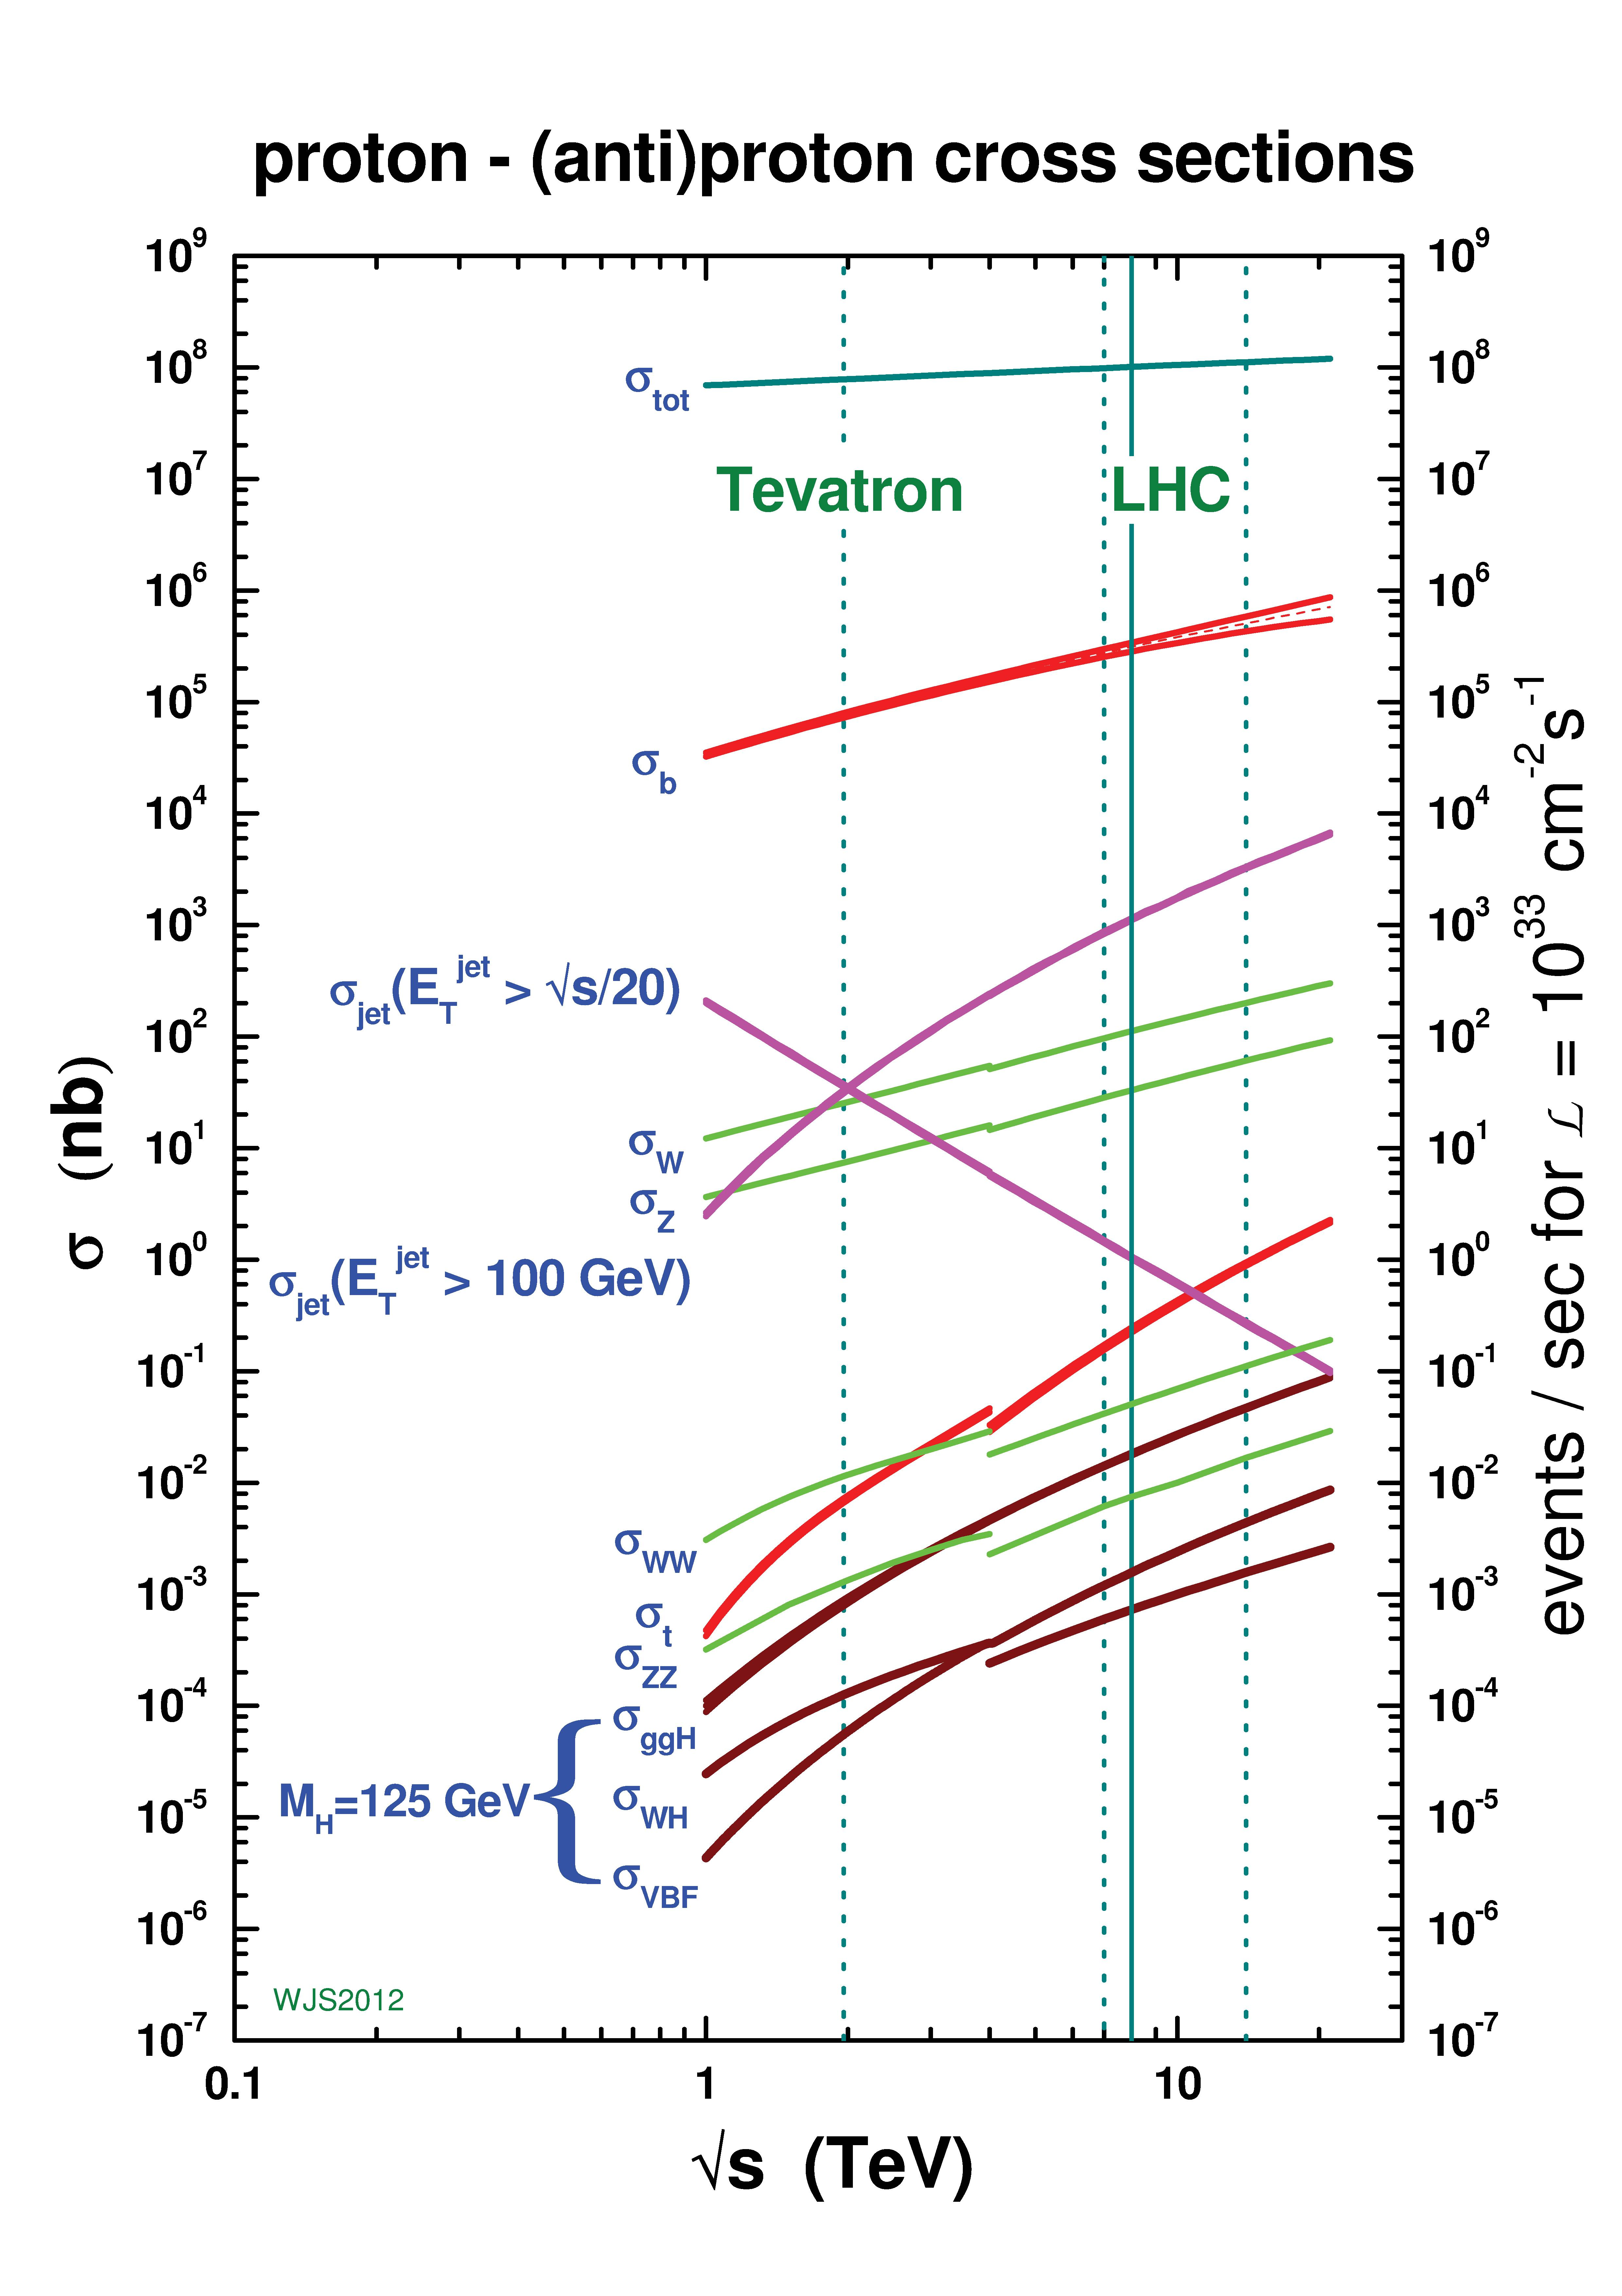
\includegraphics[scale=0.32]{images/cros.jpg}
\caption{Cross sections as a function of centre-of-mass energy \cite{<AQL>}.}
\label{fig:x cross section}
\end{figure}

\begin{figure}[h]
\centering
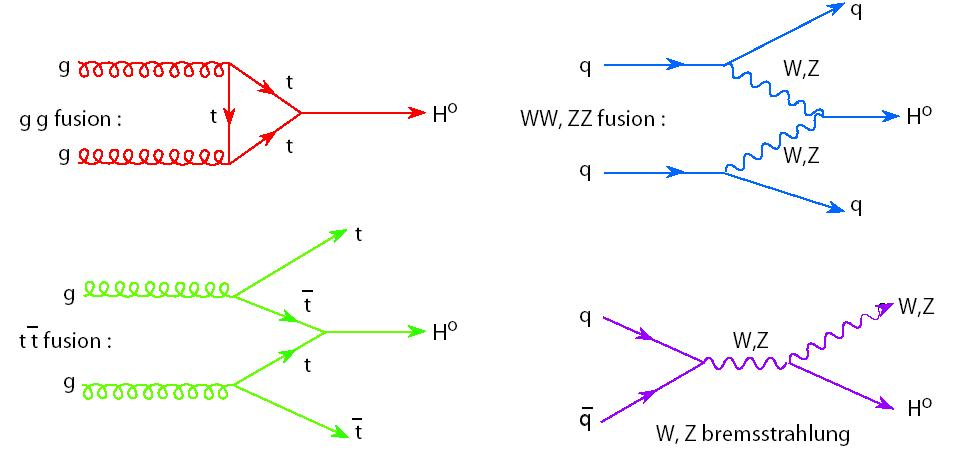
\includegraphics[scale=0.32]{images/Production Mechanism.jpg}
\caption{Feynman Diagrams For Prodcution of Higgs: (i)gluon fusion, (ii)vector boson fusion, (iii)$\Pqt\Paqt\PHiggs$ associated production, (iv)associated production with a vector boson \cite{<HPDC>}.}
\label{fig:pm}
\end{figure}

\vspace{5mm}
\textbf{GLUON FUSION} \\
In gluon-gluon fusion (ggH), two gluons merge by an intermediate quarks loop as demonstrated in Fig.\ref{fig:pm}(i), the main production mode with the largest cross section. It leads by more than one order of magnitude than the rest of the production modes as shown in Fig.\ref{fig:Cross}. This is due to the very high gluon luminosity when hadrons collide at TeV energies existing in the LHC. As top quark is the heaviest quark, its input is the largest to the loop amounting to $\sim$90\% and bottom quark accounts for other noticeable input $\sim$5-10\% out of the total cross section \cite{<PDG>}.\\
Quantum Chromodynamics corrections of higher orders are significant in this process, such as next-to-leading order(NLO) QCD corrections increase the cross sections by a factor of $\sim$2. High end computations are crucial as this thesis uses N3LO QCD and NLO EW computations \cite{<HPDGH>,<Handbook>}.

\vspace{5mm}
\textbf{VECTOR BOSON FUSION}\\
Vector boson fusion (VBF) is the next most prominent production mechanism having a cross section around an order of magnitude less than ggH as illustrated in Fig.\ref{fig:pm}(ii). This process takes place when a virtual \PZ or \PW boson is exchanged among two fermions, which fuse into Higgs boson. This mechanism has high invariant mass forward and backward energetic jets, which gives it a distinct experimental signature. The characteristic topology helps removing ggH production and Standard Model backgrounds provided by the two jets. The cross sections of leading order (LO) and NLO have \cite{<Handbook>} negligible uncertainties and QCD corrections of higher order are also very small.

\vspace{5mm}
\textbf{TOP QUARK ASSOCIATED PRODUCTION}\\
Associated production with a top and anti-top quark ($\Ptop\bar{\Ptop}$H) as displayed in Fig.\ref{fig:pm}(iii), is close to two orders of magnitude lower than ggH production and many times less than VBF production. It predominantly involves collision of two gluons, each of which decays into quark-antiquark pair. A quark and anti-quark from each of these pair, then fuse together into a Higgs boson. If the final state contains $\Ptop\bar{\Ptop}$ pair, a rare signature in experiments is seen which is used to measure this unique production mode. The QCD corrections are of the higher-order of around $\sim$1.2 and are compared at NLO EW + NLO QCD accuracy \cite{<Handbook>}.

\vspace{5mm}
\textbf{VECTOR BOSON ASSOCIATED PRODUCTION}\\
Vector boson associated production (also known as Higgs-Strahlung) also a prominent production mechanism which occurs about twice less frequently than vector boson fusion, is shown in Fig.\ref{fig:pm}(iv). In this process a pair of oppositely charged fermions fuse and generate a \PZ or \PW boson that subsequently produces Higgs boson.\\
In hardronic vector boson decays we see boosted jet pairs with fixed mass resembling vector boson's nominal mass. When there are leptonic decays, either missing transverse energy for $WH$ with one lepton or missing transverse energy for $ZH$ along with a pair of leptons are detected. The production mode has significant QCD corrections of higher order and thereby, computed with NLO EW + NNLO QCD accuracy \cite{<Handbook>}.


\begin{figure}
\centering
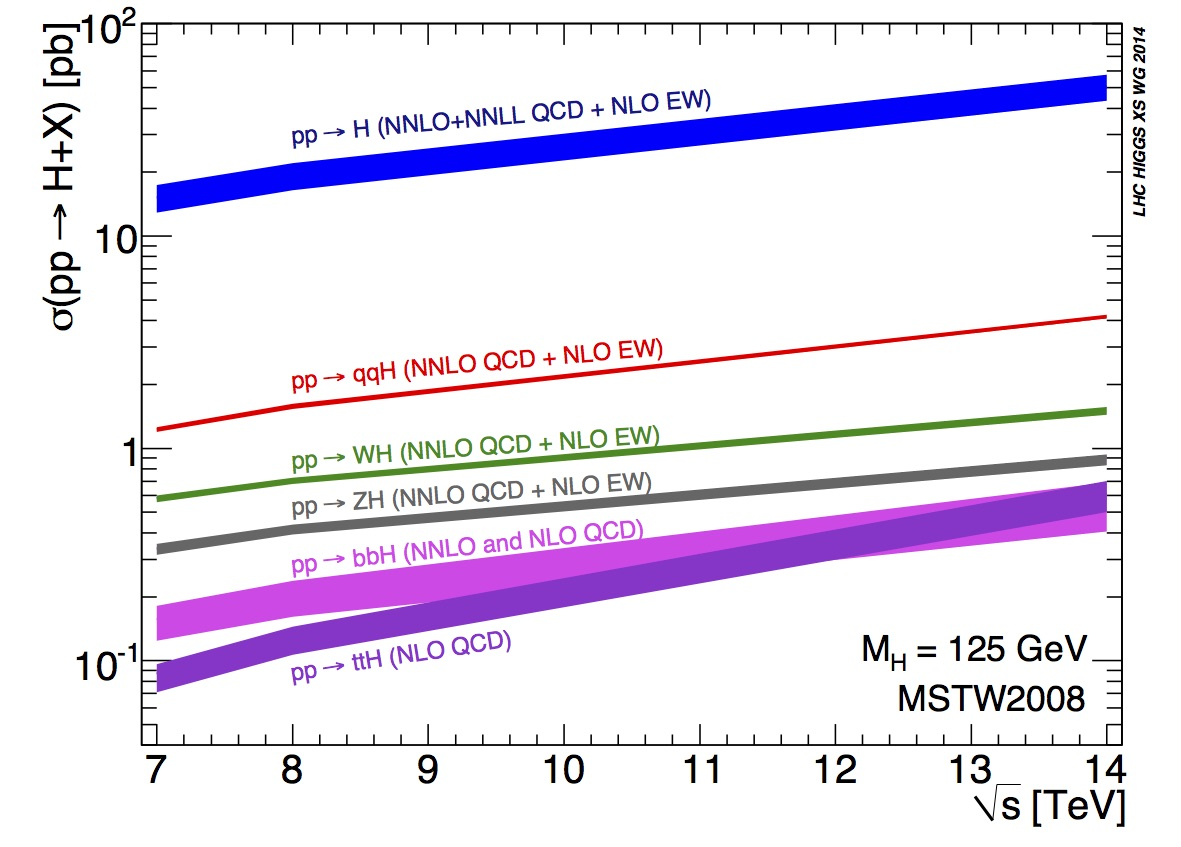
\includegraphics[scale=0.32]{images/Cross Sec.jpg}
\caption{Cross Section of Production Modes for $m_H$=125 GeV \cite{<Cross>}.}
\label{fig:Cross}
\end{figure}

\vspace{5mm}
\textbf{ADDITIONAL PRODUCTION MECHANISMS}\\
Bottom quarks associated production ($\Pqb\Paqb\PHiggs$) and production with top quark ($\Pqt\Pq\PHiggs$) are also taken into account during Higgs searches. The $\Pqb\Paqb\PHiggs$ and one of the $\Pqt\Paqt\PHiggs$ production channel have cross sections that are similar to each other, where as $\Pqt\Pq\PHiggs$ has an exclusive cross section one order of magnitude lower. Supplementary production channel of Higgs boson have even smaller cross section and hence, are not taken into consideration.

\subsection{Decay Mechanisms}
According to quantum mechanics, if a heavier particle can decay into lighter particles, then it eventually does. The probability of the decay is dependent on multiple factors, such as the strength of interactions, difference in mass, etc. SM sets parameters for these factors, except for the Higgs boson mass. For Higgs boson, the Standard Model anticipates a mean lifetime of $1.6\times10^{-22}$s at a mass of 125GeV \cite{<hb>}. The mean lifetime of decay products is used to detect the Higgs boson, as it is short-lived to reach the detector, on its own.\\
The branching ratios of the Higgs decay modes, predicted by the SM, depend on the Higgs mass value illustrated in Fig.\ref{fig:decaybr}. Since all the elementary particles interact with Higgs boson, it  can decay via many different processes. Higgs can decay through multiple processes, as it interacts with all elementary particles, such as decay to massless particles or through an intermediate virtual particles loop. Some of these are given in Table.\ref{tab:dec}.

\begin{table}[h]
\centering
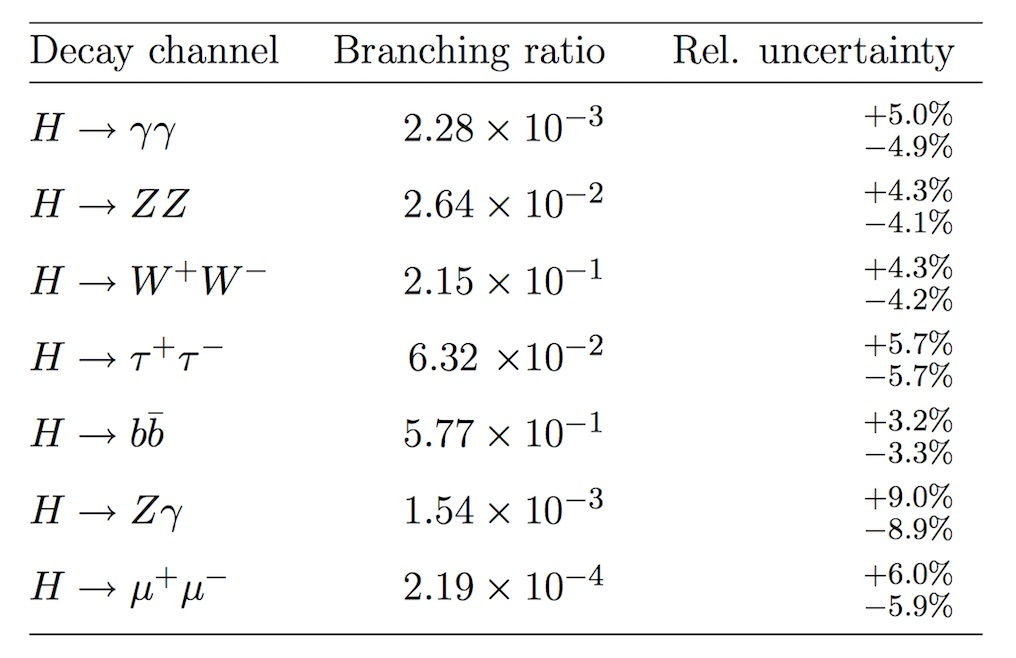
\includegraphics[scale=0.32]{images/Decay Channel.jpg}
\caption{Decay Channels of Higgs Boson \cite{<Cross>}.}
\label{tab:dec}
\end{table}

\vspace{5mm}
\textbf{DECAYS TO QUARKS AND LEPTONS}\\
The first decay we will discuss is Higgs decay into a pair of fermion and an anti-fermion. The Higgs boson interaction strength is proportional to fermionic mass therefore a decay to heavy fermions is more likely to occur as opposed to light fermions. Accordingly, then most probable decay is $\PHiggs \rightarrow \Pqt\Paqt$, although its occurrence is permitted when the Higgs boson mass is more than 2$m_t$ ($\sim$350GeV). With a branching ratio of $\sim$58\%, Higgs commonly decays to $\Pqb\Paqb$ when the mass is $\sim$125 GeV \cite{<PDG>}.\\
Subsequently, Higgs boson decaying into a fermionic pair of $\Pgtp\Pgtm$, that is probed by the decay products of tau leptons. The rest of the most likely decays to fermion anti-fermion pairs such as $\Pgmp\Pgmm$, $\Pcharm\APcharm$, $\APelectron\Pelectron$, can not be exploited yet due to their QCD background signatures or little branching ratio at present integrated luminosity.

\vspace{5mm}
\textbf{DECAYS TO GLUONS AND EWK GAUGE BOSONS}\\
For Standard Model Higgs at mass of 125 GeV, the possible decays are $\Pgg\Pgg$, $\Pg\Pg$, $\PZ\PZ^\ast$ and $\PW\PW^\ast$. In these with biggest branching ratio, $\PW\PW^\ast$ channel has a $\sim$21\% probability. Then is a gluon pair decay which occurs $\sim$8\% of the time. We can not study this decay at present in the collider because it is not distinguishable from the QCD dijet background. The decay into a photon pair is a significant channel for study and search of Higgs boson, but it lacks clear signal over background ratio. Comparatively, diphoton invariant mass has appreciable experimental resolution, where the small Higgs signal is seen as a peak over other backgrounds from either jet signals which are misinterpreted as photons or QCD production of diphotons.\\
The bosonic $\PZ\PZ^\ast$ pair decay has a low branching ratio $\sim$2.6\%, but it is completely reconstructed in the final state and its experimental invariant mass resolution is also favorable. For the final state ($H\rightarrow ZZ^{\ast}\rightarrow 4l$) a good signal over background ratio is detected as the branching ratio decreases even more for decays of $\PZ \rightarrow 4l$. This channel is popularly known as the ``golden channel'', it will be explained in detail in the next section.\ref{subsection:gc} and is mainstreamed in the following thesis.

\begin{figure}[h]
\centering
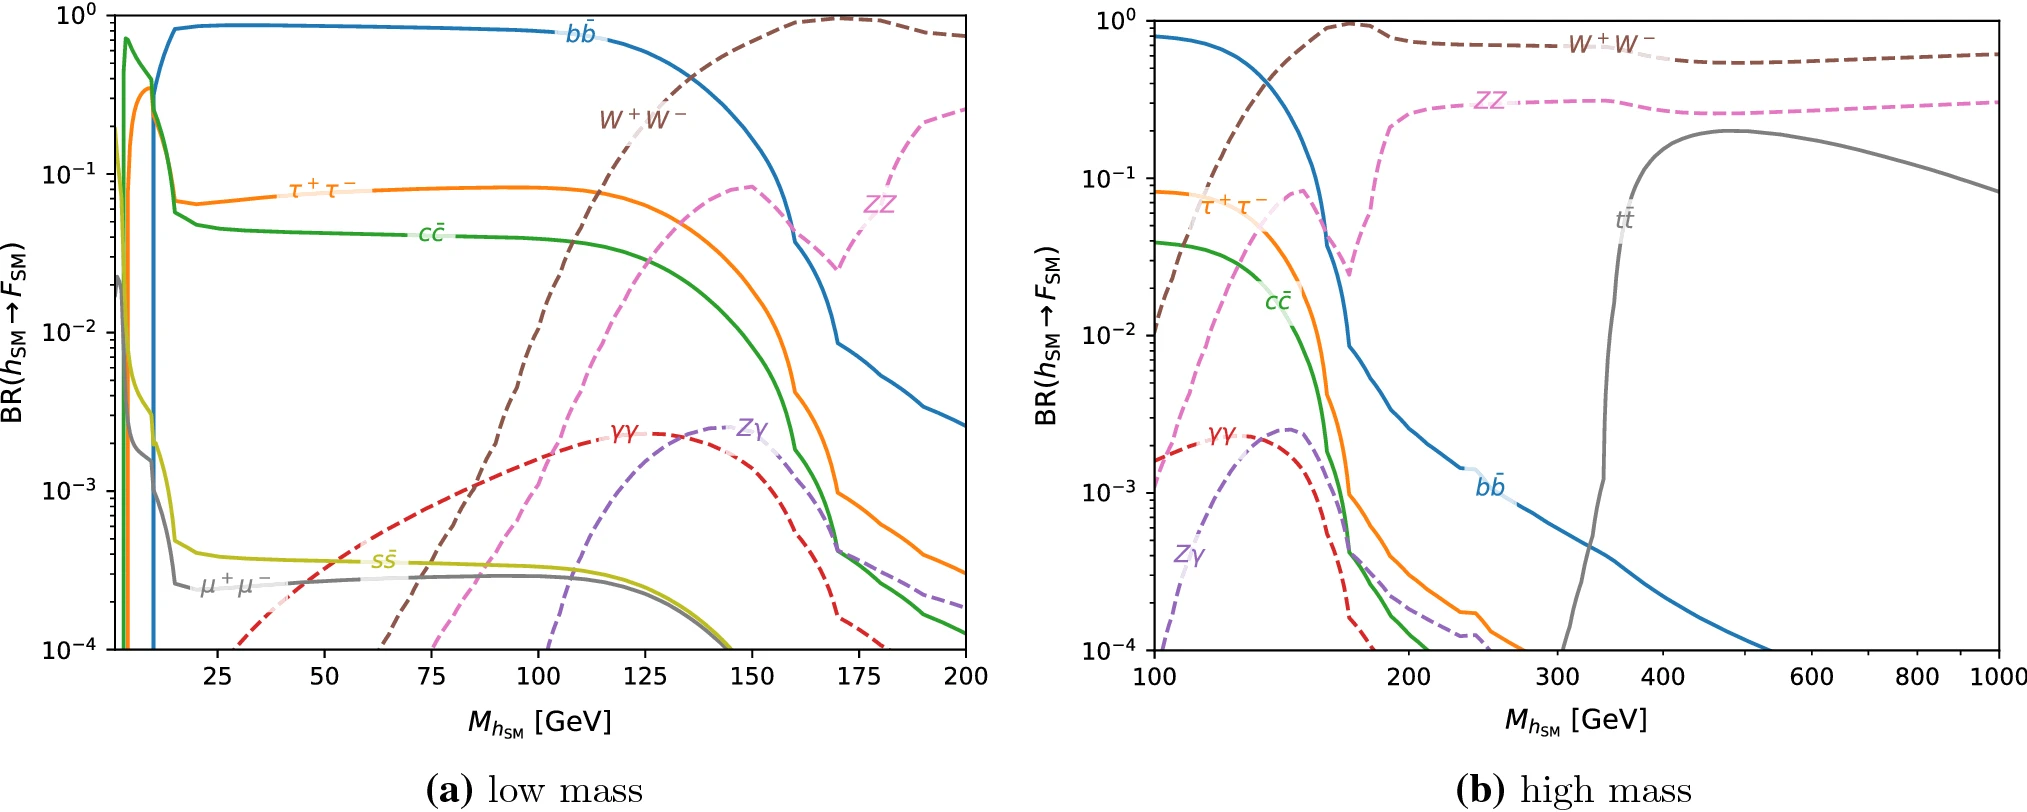
\includegraphics[scale=0.2]{images/BR.png}
\caption{Branching ratios of Higgs decay split into the low mass domain (left panel) and the high mass domain (right panel) \cite{<decaybr>}.}
\label{fig:decaybr}
\end{figure}

\subsection{Golden Channel}
\label{subsection:gc}
In golden channel, Higgs boson decays to a pair of Z vector bosons which in turn decay into electrons or muons pairs, represented as $H\rightarrow ZZ^{\ast}\rightarrow 4l$, directly as $H\rightarrow4l$. Detecting four leptons in the final state that come from Higgs boson decay in our data does not indicate a Higgs boson signal is discovered. There are Standard Model interactions that have similar signature but without the indulgence of Higgs. Most common are two Z bosons or Z\Pgammastar detected by gluon pair fusion or annihilation of quark and anti-quark pair. Another significant contribution comes from reducible background ``Z+X'', where X stands for Z boson reproduced by a pair of leptons, which are not products of Higgs.\\
4\Pe, 4\Pmu and $2\Pe2\Pmu$ are the three considered final states of the decay, with contrasting mass resolution and reducible background rate, therefore analysed separately. The four leptons in final state have a definite signature, hence varying production mechanisms are easily attainable by event jet's extra objects, absent transverse energy and additional leptons. Few of the main production mechanisms have low statistics because of low branching ratio around 0.0124\%, but in HL-LHC Run III this channel is the main tool for measuring properties and Beyond Standard Model (BSM) anomalies.\\
$H\rightarrow ZZ^{\ast}\rightarrow 4l$ is proclaimed ``golden channel'' for the final missing piece: hunt for Higgs boson of SM. The prominent reasons for which are:
\begin{enumerate}
    \item Final state objects are completely reproduced. Even at low energy LHC experiments can reproduce leptons and they can overturn four leptons from final state back to Higgs boson. To discriminate signal from background, kinematic properties of $4l$ like their four momentum are used.
    \item Exemplary momentum resolution. Higgs boson is measurable precisely with the distinct momentum resolution of electrons and muons,
    \item Notable signal to background ratio. There is a $2:1$ signal to background ratio around limited mass region of Higgs boson and low branching ratio.
\end{enumerate}
The golden channel seen in Fig.\ref{fig:golden} has given notable results from CMS and ATLAS collaborations at $\sqrt{s}=13$ TeV e.g.:
\begin{itemize}
    \item Higgs boson mass measurement, apart from the one given in the SM. \cite{<measure>}\cite{<measured>}\cite{<couple>},
    \item Width measurement \cite{<measure>}\cite{<measured>}, jointly analysed in the off-shell and on-shell areas \cite{<width>}\cite{<constraint>}, and for one taken from distance of flight in the accelerator \cite{<limit>},
    \item Signal strength, the observed rate ratio of the Higgs boson to the rate expected in SM and Higgs-fermion and Higgs-gauge boson couplings \cite{<measure>}\cite{<couple>},
    \item Spin-parity, biasing over zero spin and even parity for Standard Model consistency \cite{<measure>}\cite{<study>}\cite{<evidence>}\cite{<cons>}\cite{<diboson>},
    \item Fiducial cross section, unified and also several parameterized functions \cite{<fid>}\cite{<pro>} used in the Standard Model Lagrangian construction of the Higgs boson processes, studying tensorial couplings, uncommon production modes, in analysis of effective form factors, etc.,
    \item Anomalous couplings, interactions test via scattering amplitude of a spin-zero $H$ boson with two spin-one gauge bosons $VV$, such as $gg, \gamma\gamma, ZZ, WW$ and $Z\gamma$ \cite{<limit>}\cite{<cons>}\cite{<diboson>},
    \item Determining other heavy Higgs bosons in $H \rightarrow \Plepton \Plepton \Plepton \Plepton, H \rightarrow \Plepton \Plepton \Pnu \Pnu, H \rightarrow \Plepton \Plepton \Pq \Pq$ and $H \rightarrow \Pnu \Pnu \Pq \Pq$ with Higgs mass spectrum with upper limit extended to 1 TeV \cite{<sear>}\cite{<pair>}.
\end{itemize}
\begin{figure}[h]
\centering
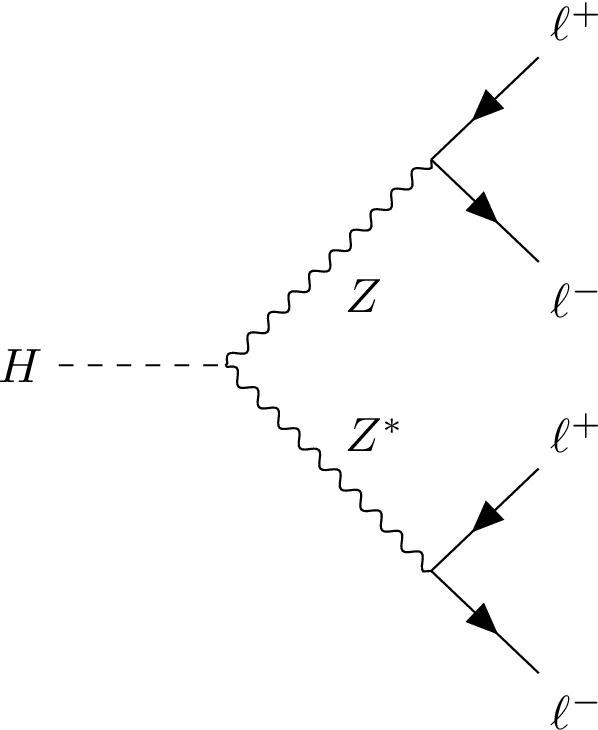
\includegraphics[scale=0.2]{images/goldenchannel.jpg}
\caption{The Golden Channel}
\label{fig:golden}
\end{figure}
\section{Experimental Searches for Higgs Boson}
This section will give brief chronicle search history which led to Higgs boson discovery declared on $4^{th}$ July in 2012 and is at present being authenticated by all purpose machine LHC. LHC's recent measurement results and current searches.
\subsection{Indirect Constraints on the Standard Model Higgs Boson}
Fits to precision measurement of electroweak observables set indirect experimental restrictions on mass of Standard Model Higgs boson. Loop effects in Higgs boson are a major factor in the \PWpm and \PZ vacuum polarization, which generates a logarithmic sensitivity on the ratio of the \PZ and \PWpm bosons masses to the Higgs boson mass. A likelihood fit to the precision electroweak samples collected during past three decades at Large Electron-Positron (LEP) Collider at CERN, Standford Linear Collider (SLC), the Tevatron at Fermilab and other results, gives $m_{H}$=$94^{+29}_{-24}$GeV or $m_{H}<152$GeV at 95\% confidence level (C.L) \cite{<pem>}. Loop effects also make top quark to contribute to the \PWpm boson vacuum polarization which has quadratic effect on the top mass. For top quark, $m_{\Pqt}$=173.2 $\pm$0.9 GeV \cite{<tew>} and for \PWpm mass of 80.385 $\pm$0.015 GeV \cite{<pem>} were considered.
\subsection{Searches for the Standard Model Higgs Boson at LEP}
Higgs-strahlung in the s-channel is the leading mechanism for acquiring Higgs boson in $\Pep\Pem$ collisions at LEP energies, $\Pep\Pem \rightarrow \PHiggs\PZ$. Final state \PZ boson is either virtual (LEP1 ), or on mass shell (LEP2). Higgs boson production via $\PWplus\PWminus$ and $\PZ\PZ$ interaction in the t-channel at LEP energies, has a small cross section. Higgs boson in LEP searches is sensitive to variation in center-of-mass energy, $\sqrt{s}$. During the LEP1 phase, mass of the SM Higgs boson was approximately 65 GeV bounded from below  \cite{<jane>}. At LEP2, data samples were generated in huge amount at $\sqrt{s}=209$GeV. At LEP1, production modes such as $\PZ \rightarrow \Plp\Plm$ and $\PZ \rightarrow \Pgn\Pagn$ were used as other channels were restricted by the backgrounds. Where as LEP2 used all decay modes in data accumulation.
\subsection{Searches for the Standard Model Higgs Boson at Tevatron}
In the Tevatron, principal production interactions were: gluon fusion $\Pg\Pg \rightarrow \PHiggs$, associated vector boson production ($\PWpm\PHiggs$ or $\PZ\PHiggs$) and vector boson fusion (VBF). Some channels were optimised for VBF because it has a smaller cross section. Compared to LEP analyses, Tevatron has lower signal-to-background ratio, although the systematic uncertainties on the calculated background signals are generally larger than the signal rates \cite{<RPP>}.
\subsection{Searches for the Standard Model Higgs Boson at LHC}
At hadron colliders, production mechanism depends on the principle of mass-Higgs coupling, i.e couples more strongly to heavy particles which are the top quark, vector bosons (\PZ, \PW) and the bottom quark. The Feynman diagrams of the four main production modes which are displayed in Fig.\ref{fig:pm} and Fig.\ref{fig:Cross}, in which dominant production process is gluon–gluon fusion mechanism. This is followed by the $\PW\PW$ and $\PZ\PZ$ fusion process, for large $m_{H}$ values it can reach $gg$ fusion cross section. The cross sections for the $\Pqt\Paqt$ pairs and associated production with \PW/\PZ bosons are one to three orders of magnitude less than the $\Pg\Pg$ pair and for mass range $m_{H}\le250$ GeV these interactions are relevant.